\chapter{Úvod do diplomovej práce}
Diplomová práca na tému "Multiplatformní aplikace pro správu síťových prvku Mikrotik" sa bude primárne zaoberať samostatným mikrotikom. Pomocou aplication programable interface (API)je cieľom  vytvorenie jej konzolovej časti (backendu) a grafickej časti (frontendu). Tieto dve časti dajú celkovú applikáciu dokopy ako celok.\\
V prvej časti práci bude definovanie Mikrotik API a jeho možností, porovnanie podobnosti s operačným systémom unix. Ďalej budú popísané možnosti zabezpečenia API pomocou secure socket layer (SSL). Budú tu tiež spomenuté použité porty,a ďalšie možnosti.\\
V druhej časti práce bude popis API a spôsoboch softvérového riešenia aplikácie pre správu Mikrotikov. Bude spomenutý aj úvod do certifikátov a to konkrétne Single Sign-on metódy.\\
V ďalšej časti bude návrh riešenia softvérovej implementácie aplikácie. Bude obsahovať popis, princípy, diagramy, hlavne Unified modeling language (UML), popisy knižníc, jednotlivých tried a modulov. Každý modul bude popísaný svojou funkcionalitou, parametrami a výstupom s praktickými ukážkami.\\
V ďalšej časti bude použitá implementácia softvérového návrhu riešenia. Bude tu riešenie ako v konzolovej časti, jeho ukážky, test a výsledky. \\
V predposlednej časti práce bude ukážka grafického spracovania konzolovej časti aplikácie a ich prepojenia do jednej aplikácie, spoločne s ukážkami kódov, testu  a výsledkov.\\
V poslednej časti sa bude nachádzať návod na inštaláciu softvéru a testovanie softvéru.
\chapter{Mikrotik a RouterOS (SwitchOS)}
V dnešných malých  a stredne veľkých firmách sa na správu siete používajú prevažne routre a switche typu Mikrotik. Mikrotik je firma vyvíjajúca routre a switche,prístupové body a ďalšie sieťové prvky vyrábané v Litve. \\
Mikrotik zariadenia používajú operačný systém routerOS, prípadne switchOS. Rozdiel medzi nimi je na základe použitého zariadenia. Čo sa týka routrov, používa operačný systém routerOS, switch používa switchOS, v prípade prístupových bodov (AP) je to routerOS. 
\section{Mikrotik API}
Za pomoci Mikrotik API môžeme programovať užívateľské programy a prostredia na riadenie a konfiguráciu Mikrotik zariadení. V dnešnej dobe existuje softvér na konfiguráciu mikrotik zariadení a to pod názvom \textbf{Winbox}. Winbox v dnešnej dobe existuje len na operačný systém Windows a Macintosh (MAC), a to len cez emuláciu windows aplikácií cez wine, podobne ako na linuxe. Bohužiaľ na operačný systém Linux winbox samostatne neexistuje a musí sa simulovať pomocou emulátoru Windows aplikácií za pomoci programu Wine. Toto spôsobuje komplikácie pri použití niektorých funkcií winboxu ale aj iných programov operačného systému Windows. Výstupom práce bude práve Graphical User Interface (GUI), v podstate upravený a zjednodušený winbox. 
\subsection{Požiadavky na použitie API}
\begin{itemize}
\item Verzia routerOS verzie \textit{3.0.X} a vyššie \cite{API}
\end{itemize}
\subsection{Porty}
Základné porty na použitie Mikrotik API \cite{API} sú:
\begin{itemize}
\item \textbf{API port}: 8728
\item \textbf{Application programable interface Secure Socket Layer (API-SSL) port}: 8729
\end{itemize}
\subsection{Základný port 8728}
Na základné pripojenie k API aplikácii na prvku Mikrotik musí byť povolený port 8728, ktorý tiež nájdeme v IP-> Services spoločne s API-SSL.\\
Na základné pripojenie nie je potreba žiadneho transport layer security (TLS) certifikátu. Stačí jednoducho napísať kód a skompilovať ho. 
\subsection{SSL port 8729}
Pre použitie portu 8729 tiež známeho ako API-SSL portu je potreba zabezpečenej komunikácie pomocou SSL protokolu. \\
Primárne muisú byť natavený port, základný port 8729 v IP -> Services. Môžeme ale definovať aj užívateľsky definovaný port. \\
Možnosti nastavenia API-SSL:
\begin{itemize}
\item prístup bez certifikátu TLS
\item prístup pomocou certifikátu TLS
\end{itemize} 
\subsubsection{Prístup pomocou certifikátu TLS}
Pre použitie certifikátu TLS je potrebné vygenerovať certifikát TLS, a to na certifikačnej autorite alebo na ľubovoľnej linux stanici ideálne, ale tiež to dokážeme spraviť aj na Windows stanici či MAC. 
Spôsoby vygenerovania certifikátov:
\begin{itemize}
\item openssl
\item easy-rsa 
\item Windows Server Certificate Services
\end{itemize}
\subsubsection{Openssl}
Openssl \cite{OpenSSL} je softvér na generovanie certifikátov pre komunikáciu v počítačovej sieti. Koreňovo sa používa na prístup na web skrz protokol Hyper Trasfer Transport Protocol Secure (HTTPS). Pre vygenerovanie certifikátov sa musí vygenerovať: \begin{itemize}
\item certifikát \textit{*.crt}
\item certifikačný požiadavok \textit{*.csr}
\item kľúč k certifikátu \textit{*.key}
\end{itemize}
\subsubsection{Easy-rsa}
Softvér easy-rsa \cite{EasyRSA} sa používa na vytvorenie open-source certifikačnej autority a užívateľých certifikátov napr. pre potreby HTTPS spojenia.\\
Po nainštalovaní easy-rsa napr. na Ubuntu príkazom \textit{sudo apt install easy-rsa} sa musí spraviť nasledovné: \begin{itemize}
\item Nakopírovanie konfiguračných súborov do zložky autority
\item Vytvorenie šablóny na vygenerovanie certifikačnej autority
\item Vytvorenie užívateľksých certifikátov
\end{itemize}
\subsubsection{Active Directory Certificate Services}
Windows riešenie \cite{WindowsCA} pre generovanie  certifikačnej autority je inštalácia roly servera Active Directory Certificate Services. \\
Pre použitie certifikačnej autority na Windows servery je potreba:
\begin{itemize}
\item Inštalácia role serveru
\item Nadefinovanie certifkačnej autority
\item Generovanie certifikátov
\end{itemize}
\section{API slová}
\label{chap:APIwords}
API slová \cite{API} sú základnou časťou API "vety". API "veta" predstavuje príkaz v pouužití príkazu napr. \textit{\//ip/address/print}, \textit{\//ip/address/add address="10.1.1.1/24" interface="ether1"}. \\
Parametre na slová:
\begin{itemize}
\item každé slovo má svoju zakódovanú dĺžku t.j. 
\begin{itemize}
\item 0 - 127 bitov zaberá 1 Byte
\item 128 - 1023 bitov zaberá 2 Byty 
\item 1024 bitov - 2097 kib zaberá 3 Byty
\item viac ako 2098 kib zaberá 4 Byty
\end{itemize}
\item jednotlivé slová súzaradené do viet
\item maximum bztov na slovo sú 4 Byty
\item kontrolné byty sa nepoužívajú
\end{itemize}
\section{Príkazové slová API}
Slová Mikrotik API sa zaraďujú do API viet použitím API slov, na ktoré platia požiadavky, ktoré sú spomenuté v kapitole \ref{chap:APIwords}.Na použitie API viet je potreba začínať znakom \textit{\//}. Napr. miesto \textit{ip address print} sa použije \textit{\//ip/address/print}.\\
Pre úplnosť API viet musí platiť \cite{API}
\begin{itemize}
\item zakódovaná dĺžka slova
\item slovo musí začínať znakom \//
\item musí byť použitá správna syntax
\end{itemize}
\section{Použitie atribútov v príkaze a filtrovanie}
V prípade konfigurácie mikrotik zariadení sa pre nastavenie jednotlivých prvkov používajú tzv. atribúty \cite{API} napr. ip adresa, číslo pravidla, meno rozhrania, nastavenie virtuálnej lokálnej sieti (VLAN). \\
Použitie atribútov má špeciálnu syntax pre konfiguráciu prípadne zmenu prvku na mikrotiku, prípadne pridanie a zmazanie prvku. Na použitie atribútov sa použije špeciálny znak \textit{=}. Napr. \textit{\//ip/address/add =address=10.1.1.1/24 =interface=erher1}.\\
Pre filtrovanie prvkov v rámci mikrotik API syntaxe sa používa špeciálny atribút parameter so znakom \textit{?}. Napr. \//ip/address/print =?type=ether1 vyfiltruje len rozhranie ether1.
\section{Špeciálne slová API}
Miktotik API má možnosť tzv. špeciálnych slov \cite{API}. Špeciálne slová sú slová, ktoré sú rezervované  a nesmú sa použiť pre iné použitie ako napríklad meno premennej, metódy, triedy, a iné. Medzi špeciálne slová patria:\begin{itemize}
\item prihlásenie sa na zariadenie \//login
\item ukončenie spojenia na zariadenie \//cancel
\item odhlásenie sa zo zariadenie \//logout
\item získanie všetkých parametrov \//getall
\end{itemize}   
\chapter{Pripojenie na Mikrotik}
\section{Možnosti pripojenia}
Pripojenie na mikrotik je realiyované pomocou niekoľkých typov softvéru:\begin{itemize}
\item \textbf{Winbox} - základný softvér na konfiguráciu mikrotiku
\item \textbf{Webfig} - konfigurácia mikrotiku pomocou webového rozhrania štandardne na portoch 80 a 443
\item Riadenie mikrotiku pripojením na mac adresu - \textbf{mactelnet}
\item Pripojenie pomocou protokolu \textbf{SSH} - zabezpečené a šifrované spojenie
\item Pripojenie pomocou protokolu \textbf{telnet} - nebezpečné v dnešnej dobe
\end{itemize}
\section{Pripojenie pomocou winboxu}
Winbox\cite{winbox} je nástroj na administráciu mikrotiku. Medzi jeho vlastnosti patrí:\begin{itemize}
\item GUI nástroj (klikátko)
\item rýchlosť
\item spoľahlivosť 
\end{itemize} 
Winbox je prepis konzolovej aplikácie do grafickej. Obsahuje tiež nástroje ktoré sa v konzole nedajú odsimulovaťnapr. graphs, torch, netmon, scheduler,...\\
Niektoré funkcie nevieme meniť pomocou winboxu napr. Media Access Control (MAC) adresu rozhrania. 
\begin{figure}[H]
\centering
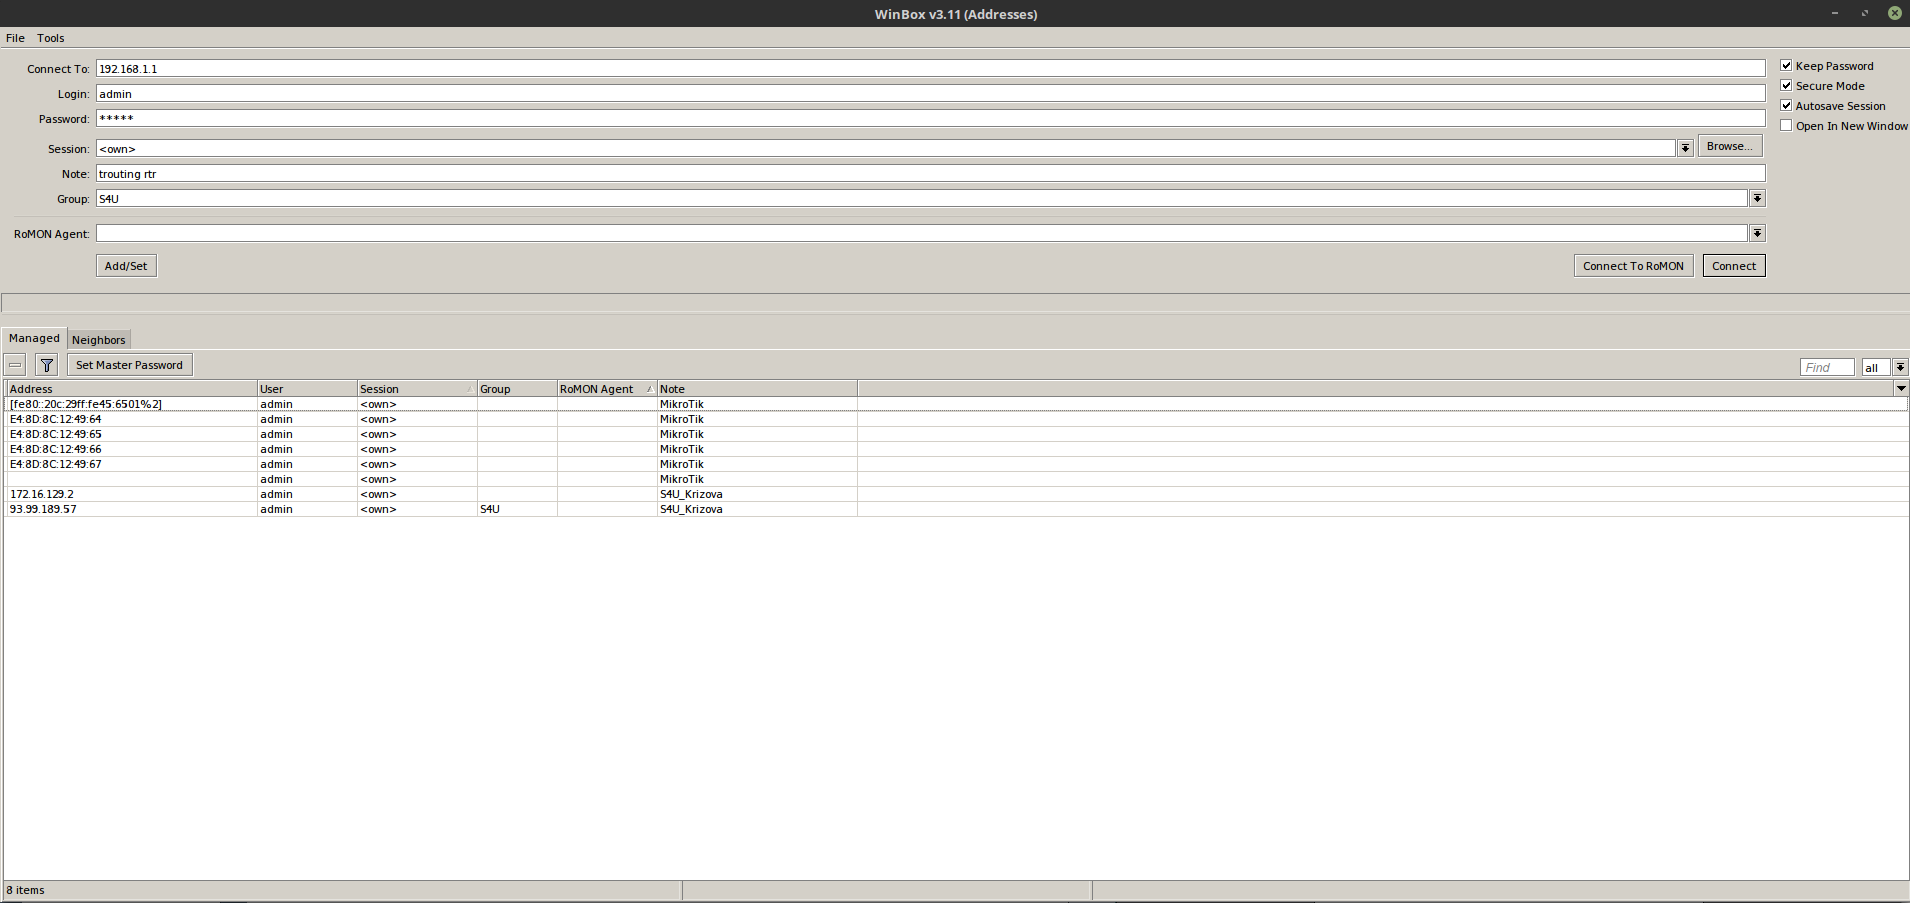
\includegraphics[scale=0.2]{../text/winbox.png}
\caption{Winbox základné prihlasovacie rozhranie}
\label{fig:winbox}
\end{figure} 
Režimy winboxu:\begin{itemize}
\item jednoduchý režim - obsahuje na pripojenie len užívateľské meno, heslo a adresu mikrotiku
\item pokročilý režim - možnosť pridania skupiny mikrotikov, popisky a názov spojenia
\end{itemize}
\section{Pripojenie pomocou webfigu}
Webfig\cite{webfig} je webová aplikácia RouterOS a umožňuje konfiguráciu, minitoring a údržbu prvkov RouterOS. Medzi hlavné tasky webfigu patrí:\begin{itemize}
\item konfigurácia mikrotiku
\item mnotring mikrotiku
\item riešenie problémov na mikrotiku za pomoci webového rozhrania
\end{itemize}
\begin{figure}[H]
\centering
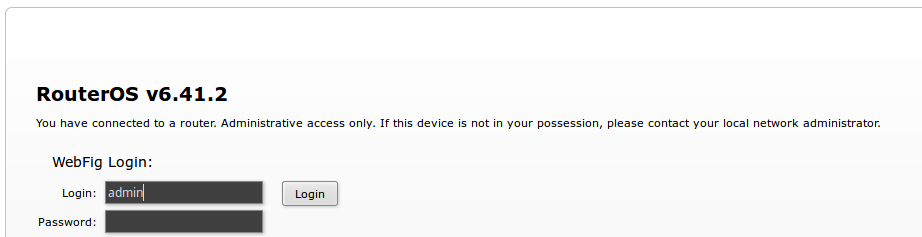
\includegraphics[scale=0.4]{../text/webfig.png}
\caption{Webfig základné prihlasovacie rozhranie}
\label{fig:webfig}
\end{figure} 
\section{Mactelnet}
Mactelnet\cite{mactelnet} predstavuje aplikačný protokol riadený na druhej vsrtve referenčného modelu. Tiež predtavuje kombináciu winboxu  a telnetu v jednom protokole. Riadi prístup na napr. nový mikrotik, ktorý ešte neobsahuje žiadnu konfiguráciu. Pracuje absolútne rovnakým spôsobom ako telnet. Je možné sa pripojiť len na fyzicky pripojený mikrotik pomocou mactelnet, vzdialený prístup pomocou mactelnet nie je možný. 
\begin{figure}[H]
\centering
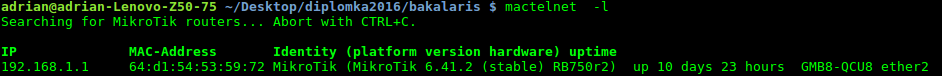
\includegraphics[scale=0.4]{../text/mactelnet.png}
\caption{Výstup príkazu mactelnet}
\label{fig:webfig}
\end{figure}
Po pripojení na mikrotik pomocou mactelnet sa nastaví základná konektivita a pripájame sa potom na základe Internet Protocol (IP) adresy. 
\section{Pripojenie pomocou telnet a SSH}
Ďalšou možnosťou pripojenia na mikrotik je prihlásenie sa pomocou telnetu\cite{telnet} prípadne SSH\cite{ssh} na konzolu mikrotiku. Napríklad na nastavenie fronty,firewallu,... .
\subsection{Pripojenie cet telnet}
Telnet predstavuje protokol, ktorý umožňuje pripojenie na vzdialené servery. Jeho štandardným portom je port 23. \\
Na povolenie pripojenia pomocou telnetu je potrebné povoliť službu telnet na mikrotiku v IP -> Services. Pre bezpečnostné účely by sa telnet nemal používať, je terčom útokov nakoľko je nešifrovaný. Pokiaľ chceme povoliť telnet na pripojenie na mikrotik, by sa mal minimálne zmeniť štandardný port z 23 na užívateľsky definovaný port.\\
Príklad príkazu na pripojenie na zariadenie pomocou telnetu: \textit{telnet <IP adresa> <port>} 
\subsection{Pripojenie pomocou ssh} 
SSH predstavuje protokol, ktorý umožňuje vzdialené pripojenie pomocou tohoto protokolu. Používa štandardný port 22. Tak isto ako u telnetu, pre SSH platí to isté, je potrebné ho povoliť v IP -> Services. SSH na rozdiel od telnetu je ale šifrovaný  a zabezpečený protokol. SSH predstavuje bezpečnú verziu telnetu. Je možné si zabezpečiť SSH prístup na bezpečnejší, a to tak, že sa budú porovnávať verejný  a súkromný kľúč certifikátu TKIP. V7stupom pripojenia SSH na mikrotik je na obrázku \ref{fig:ssh}. 
\begin{figure}[H]
\centering
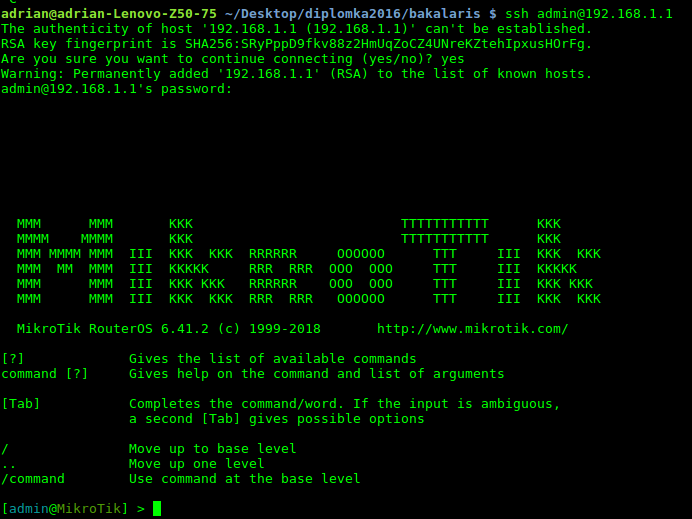
\includegraphics[scale=0.4]{../text/ssh.png}
\caption{Prihlásenie na mikrotik pomocou príkazu SSH}
\label{fig:ssh}
\end{figure}
\chapter{Programovací jazyk Python}
Python je interpretovaný, interaktívny, objektovo-orientovaný a vysoko-úrovňový programovací jazyk.Jazyk Python bol vytvorený pánom  Guido van Rossum v Wiskundskom centre informatiky v 80-tych rokoch. \\
Medzi jeho vlastnosti patrí:\begin{itemize}
\item dynamické typovanie
\item konzolové aplikácie
\item objektové aplikácie
\item všetko v pythone je objekt
\item jednoduchá syntax
\item biele znaky sú súčasťou jazyka
\item dynamické typy premenných
\item široká škála knižníc
\item dokumentácia na vysokej úrovni\
\item používaný  na webové aplikácie, strojové učenie, teórie zložitosti,...
\end{itemize}
Verzie jazyku Python:\begin{itemize}
\item Python verzia 2
\item Python verzia 3
\end{itemize}
\section{Python 2}
Vlastnosti jazyku Python 2\cite{Python2}
\begin{itemize}
\item automatická spáva pamäti (garbage collector)
\item podporuje viac vstupných paradigiem
\item Volanie niektorých príkazov je odlišné od Python 3
\item referenčný interpret sa nazýva CPython a spravuje ho organizácia Python Software Foundation
\item Súčasne sa používa Python vo verzii 2.7.2
\end{itemize}
\section{Python 3}
Vlastnosti jazyku Python 3\cite{Python3}\begin{itemize}
\item V niekorých častiach syntaxe v porovnaní s jazykom Python 2je trošku odlišná (napr. príkaz print,...)
\item Od verzie 3.6 má premenná typu slovník interné zachovávané poradie vkladaných prvkov
\item Pridanie anotácií cez metatriedy
\item deklarácia nelokálnej premennej vonku z funkcie
\item Slová typu True, False a None sú rezervované slová
\item Mnoho vlastností ma rovnakých ako Python 2
\item Miesto <> sa voverzii 3 používa relačný operátor !=
\item od Júla 2018 by mala výjsť verzia Python 3.7 s ďalšími novinkami 
\end{itemize}
\section{Prostredia na programovanie v jazyku Python}
Na realizovanie python programu je nutnosť mať nainštalovaný softvér na komppiláciu softvéru napísaného v jazyku Python. Na tieto účely slúži tzv. intergrated developement envinroment (IDE). Ecistuje niekoľko ciet aj mimo IDE ako spustiť kód napísaný v jazyku python.\begin{itemize}
\item Napísanie kódu napr. v textovom editore typu nano, vim, gedit ale aj windows riešenie ako napr. notepad
\item nainštalovaný python kompilátor
\item spustenie programu príkazom python <názov.py>
\end{itemize}
\section{Pycharm}
Pycharm predsatvuje IDE na pokročilé aplikácie napísané v jazyku Python. Exustuje v dcoch verziách:\begin{itemize}
\item Pycharm Community Edition - voľne dostupné, nelicencované, neobsahuje niektoré doplnky professional verzie
\item Pycharm Professional Edition - licencované, voľne dostupné na 30 dní, licencované, plný prístup ku všetkým doplnkom
\end{itemize}
Na nainštalovanie pycharm ľubovoľnej verzie je potreba:\begin{itemize}
\item Stiahnutie bin respektíve exe súboru inštalátoru
\item Napojenie na pracovný adresár projektu
\item Napojenie na tzv. envinroment, to je použitie cesty k volaniu príkazu python respektíve python3
\end{itemize}
Po spustení programu Pycharm sa vytvorí projekt, kde po jeho inicializácii nájdeme podobný výstup.
\begin{figure}[H]
\centering
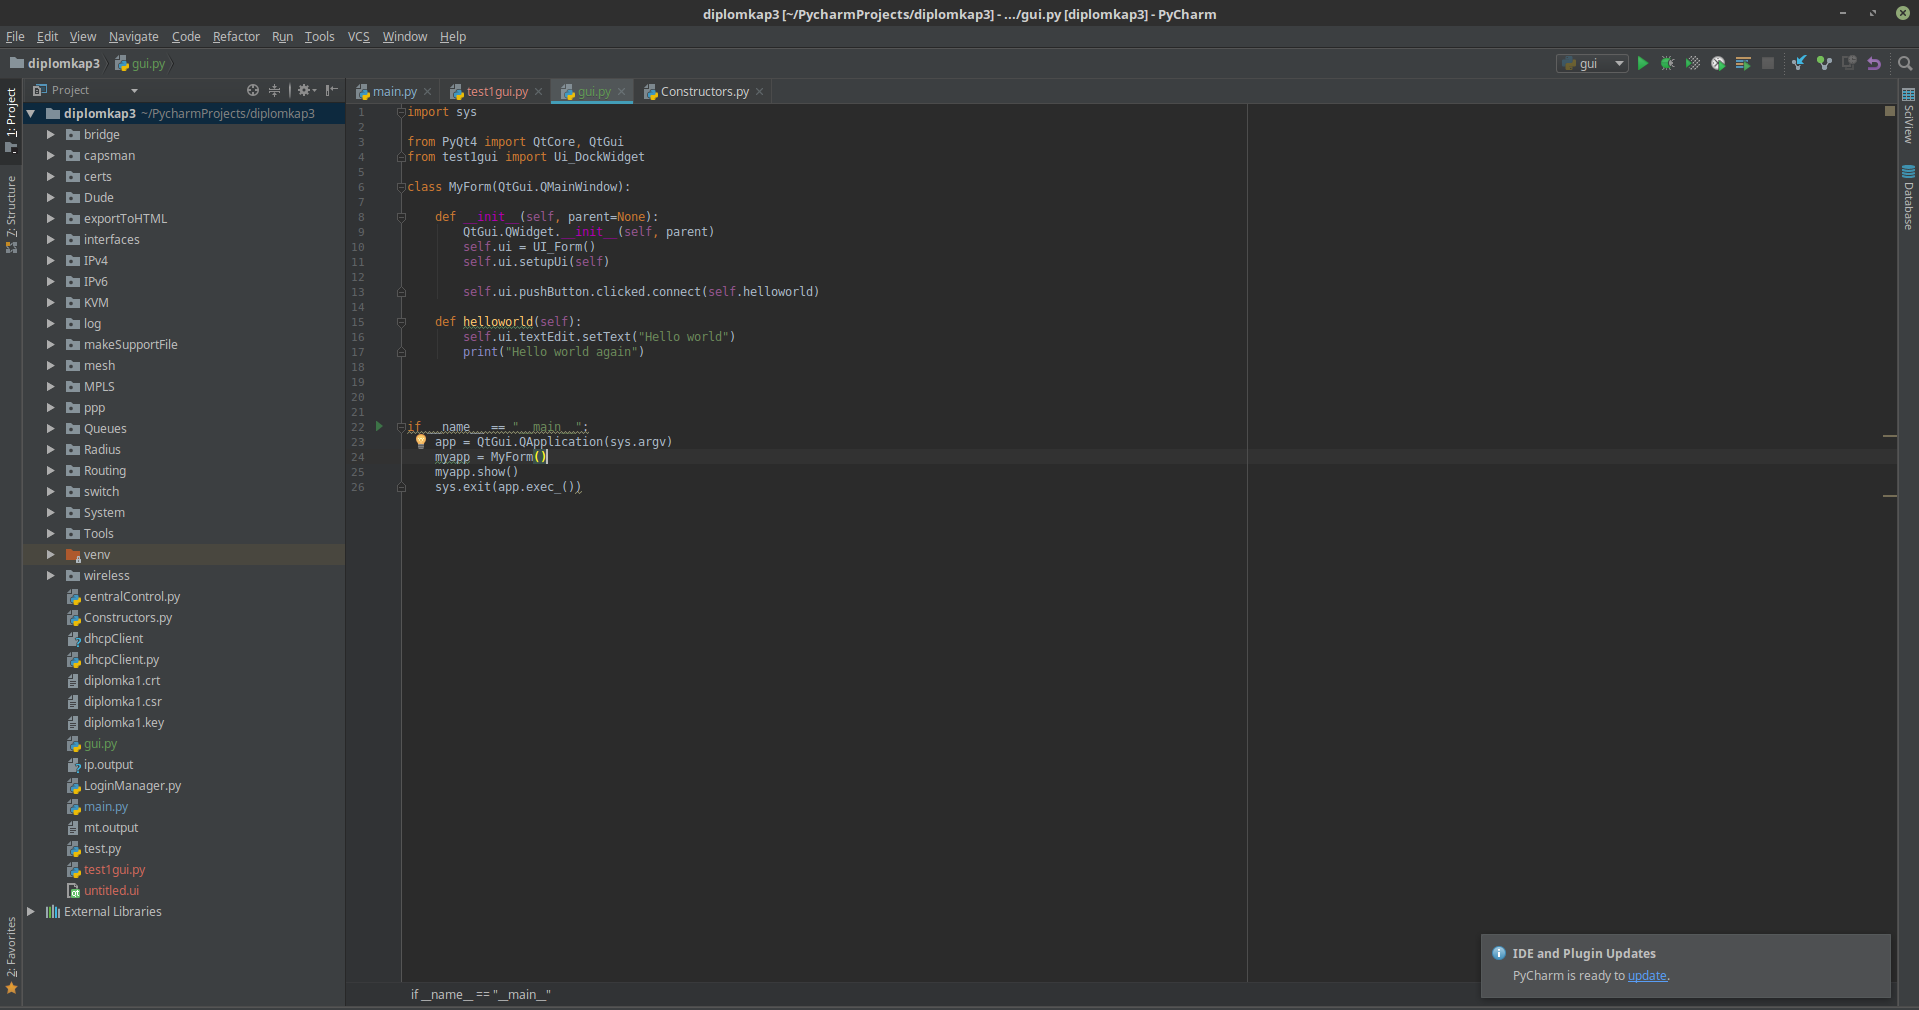
\includegraphics[scale=0.25]{../text/pycharm.png}
\caption{Rozhranie IDE Pycharm Professional Edition}
\label{fig:webfig}
\end{figure} 
Jednou z najväčších výhod je generovanie UML diagramov z kódu.
\chapter{Použité knižnice v diplomovej práci}
\section{OS.SYSTEM}
Modul operačný systém (OS) \cite{OS} je zahrnutý v rámci štandardných knižnícv jazyku python. Jeho hlavnou výhodou je použitie príkazov operačného systému na ktorom beží python.Najčastejšie sa volá príkazom os.system('príkaz').
Použitie modulu aplikujem v rámci diplomovej práce. Používa sa hlavne pri vyhľadávaní a pripájaní sa na mikrotiky pomocou protokolu mactelnet. Jeho výstup môžeme aplikovať na:\begin{itemize}
\item Štandardný výstup do konzoly
\item Výstup do osobitného súboru, ktorý sa potom ďalej spracuje
\end{itemize}
V rámci práce som tento modul použil v rámci knižnice loginManager, kde v metódach pre mactelnet vyhľadáva mikrotiky za pomoci protokolu mactelnet a ukladá to do textového súboru mt.output. \\
Nie je potreba inštalácie modulu  OS, pretože je zahrnutý v rámci štandardných knižníc jazyku python. V kóde vidíme ukážku metódy,ktorá vylistuje zoznam mikrotik zariadení za pomoci funkcie mactelnet a jej návratovou hodnotou je list zoznamu mikrotik zariadení
\begin{lstlisting}[language=python, frame=single, caption=Metóda na vyhľadanie MAC adries mikrotikov, captionpos=b]
def listMikrotikDevices(self):
 deviceList = []
 loadMacAddress = False
 os.system("mactelnet -l -t 20 2>&1 > mt.output")
 with open( "mt.output", "r" ) as file:
 for line in file:
  if loadMacAddress:
   macAddress = line.split( )[1]
   deviceList.append( macAddress )
  else:
   header = line.split( )
    if len( header ) > 1:
     if "IP" in header[0] and "MAC-Address"in header[1]:
      loadMacAddress = True
 return deviceList
\end{lstlisting}
\section{Telnetlib}
Telnetlib \cite{telnetlib} obdobne ako OS knižnica je vstavaná knižnicaprogramovacieho jazyku python. Knižnice \textit{telnetlib} implementuje protokol telnet do pythonu, definovaného referenčným modelom RFC 854. V rámci definície modulu telnetlib sa používa hlavičkový súbor \textit{telnet.h} s odstráneným záhlavým obsahujúcim \textit{TELOPT\_}. \\Modul telnetlib predstavuje jednoduchého telnet klienta pripájajúceho sa na telnet server. Na vytvorenie spojenia je potreba nasledujúcich krokov:
\begin{itemize}
\item vytvorenie objektu telnetlib s parametrami \textit{host},čo predstavuje IP adresu telnet serveru, \textit{port}, štandardne 23, nepovinným parametrom je \textit{timeout}. 
\item Je nutné otvoriť spojenie metódou \textit{open()}
\item ďalej metódami readuntil() a write() vyžadujeme očakávaný výstup a odoslanie dát na server (príkazov)
\item potom ukončíme spojenie metódou close()
\end{itemize}
Medzi najpoužívanejšie metódy v rámci diplomovej práce sú použité:
\begin{itemize}
\item  \textit{Telnet()}
\item \textit{readuntil()} -očakávanie výstupu serveru
\item \textit{write()} - zápis príkazov
\item \textit{sleep()} - doba trvania odoslania príkazu v sekundách
\item \textit{close()} - ukončenie spojenia
\end{itemize}
\begin{lstlisting}[language=python, frame=single, caption=Použitie knižnice telnetlib, captionpos=b, showstringspaces=false]
def loginTelnet(self, password, login="admin"):
 import telnetlib
 central = centralControl(login, password)
 server_list = central.listMikrotikDevices()
 print(server_list)
 for server in server_list:
 try:
  telnetcon = telnetlib.Telnet( host=server, port=23 )
  telnetcon.read_until( b"Login: " )
  telnetcon.write( login.encode( ) + "\n" )
  telnetcon.read_until( b"Password: " )
  telnetcon.write( password.encode( ) + b"\n" )
  time.sleep( 10 )
  telnetcon.close( )
 except:
  print( "Cannot connect to router via telnet" )
\end{lstlisting} 
\section{Pxssh a pxexpect}
Moduly pexpect\cite{pexpect} a jeho submodul pxssh\cite{pxssh} sú knižnice, ktoré slúžia na vyžadovanie určitého výstupu zariadenia, na to slúži knižnica \textit{pexpect} a na pripojenie sa na server z pythonupomocou protokolu SSH slúži knižnica \textit{pxssh}\\
Pexpect je čistá python modulna kontrolu a riadenie aplikácií. Pozostáva z dvoch krokov:\begin{itemize}
\item Vyžadovanie výstupu
\item Odoslanie požadovaného výstupu
\end{itemize} 
Pexpect môže byť použitý na interaktívne aplikácie, ktoré používajú protokoly SSH, File transfer protocol (FTP), telnet,atď. Pre implementáciu pexpect nie je potreba importovania knižníc z jazyka C na skompilovanie do jadra. Pracujú na všetkých platformách, a to v podobe štandardného vstupu a výstupu v príkazovom riadku operačného systému, či už serveru ale aj klienta. Pexpect je jednoduchýna implementáciu.\\
Pxssh predtavuje submodul modulu pexpect. Na zavolanie submodulu pxssh je nutné prednostne zavolať metódu \textit{spawn()}. Po vytvorení spojenia metódou \textit{spawn()} je nutné použiť metódy \textit{login()}, \textit{spawn()}a \textit{logout()}.
\subsection{Inštalácia pexpect}
Pexpect je súčasťou sady nástrojov Pypi. Aktuálna verzia modulu pexpect je verzia 4.4. Požiadavky na softvér:\begin{itemize}
\item Python vo verzii 2.7 alebo 3.3 a vyššie
\item pre windows je potreba inštalácie modulu POSIX pre jeho funkčnosť
\end{itemize}
Na nainštalovanie pexpect \cite{pexpectinstall} na linuxe,sa v príkazovom riadku zadá:
\begin{lstlisting}[language=python, frame=single, caption=Inštalácia Pexpect, captionpos=b]
pip install pexpect
pip3 install pexpect
\end{lstlisting}  
Pre inštaláciu na operačnom systéme Windows je potreba maťnainštalovaný program python prípadne python3 externe, pretože nie je štandardne zahrnutý v balíčkoch operačného systému.\\
Modul pexpect zahŕňa modul pxssh a nie je potreba ho potom extra inštalovať.\\
Nižšie vidíme ukážku použiia kombinácie modulov pexpect a pxssh na pripojenie na mikrotik.
\newpage
\begin{lstlisting}[language=python, frame=single, caption=Použitie pxssh na pripojenie na router cez protokol SSH, captionpos=b]
def loginSSH(self, server,login, password):
 from pexpect import pxssh, spawn, expect
 import getpass
 try:
  connect = pxssh.pxssh( )
  server = '172.16.49.2'
  login = 'admin'
  password = 'admin'
  port = 22
  connect.login( server, login, password )
  commands = pxssh.spawn( )
  time.sleep( 10 )
 except pxssh.ExceptionPxssh as e:
  print( "Error" )
  print( str( e ) )
\end{lstlisting}  
\section{TikApy}
\label{sec:tikapy}
Na správu mikrotik smerovačov je potreba implentovať do pythonu modul tikapy\cite{tikapy}. Modul tikapy funguje voverzii pythonu 3 a vyššie. Podobne ako bolo spomenuté v kapitole \ref{chap:APIwords}, API pracuje na základe tzv. "slov". Slová predstavujú jednotlivé príkazy na mikrotiku. Tieto príkazy budú popísané v ďalších kapitolách diplomovej práce.\\
Modul tikapy ako celkovo mikrotik API komunikuje nezabezpečene na porte 8728 a pomocou API-SSL na porte 8729. Na pripojenie sa na mikrotik pomocou modulu tikapy, ktorýmá v sebe zahrnutých mnoho knižníc na komunikáciu s mikrotikom. Medzi najčastejšie patria:\begin{itemize}
\item vytvorenie objektu TikapyClient prípadne TikapySSLClient
\item \textit{login()} - prihlásenie sa na mikrotik pomocou API
\item \textit{talk()} - odosielanie príkazov na mikrotik
\item  \textit{close()} - ukončenie spojenia
\end{itemize} 
Na nainštalovanie tikapy do pythonu je potreba to nainštalovať nasledovne, v príkazovom riadku zadíme príkaz:
\begin{lstlisting}[language=python, frame=single, caption=Inštalácia tikapy,  captionpos=b]
pip install tikapy
pip3 install tikapy
\end{lstlisting}
V rámci vytvorenia objektu sú dve možnosti:\begin{itemize}
\item vytvorenie klienta a to buď SSL klienta prípadne štandardného klienta TikapyCLient(adresa,port), pre SSL klienta to je port 8729, pre štandardného klienta port 8728
\item vytvorenie metódy login(užívateľ,heslo)
\item odoslanie príkazu metódou \textit{talk(['príkaz'])} 
\end{itemize}
Nižsie vidíme príklad metódy spoločne s konštruktorom triedy na pridanie IP adresy s príkladom použitia API slov.

\begin{lstlisting}[language=python, frame=single, caption=Príklad použitia tikapy,  captionpos=b]
from tikapy import TikapyClient
from tikapy import TikapySslClient
class Addresses:
    def __init__(self,address,username,password):
        self.client = TikapySSLClient( address, 8729 )
        self.client.login( username,password)
    def addAddress(self,address,interface):
     """
     Method will add address
     :param address:
     :param interface:
     :return:
     """
     ipv4 = self.client.talk(['/ip/address/add',
     '=address='+address,'=interface='+interface])
     return ipv4
\end{lstlisting} 





